\documentclass[]{article}
\usepackage{lmodern}
\usepackage{amssymb,amsmath}
\usepackage{ifxetex,ifluatex}
\usepackage{fixltx2e} % provides \textsubscript
\ifnum 0\ifxetex 1\fi\ifluatex 1\fi=0 % if pdftex
  \usepackage[T1]{fontenc}
  \usepackage[utf8]{inputenc}
\else % if luatex or xelatex
  \ifxetex
    \usepackage{mathspec}
  \else
    \usepackage{fontspec}
  \fi
  \defaultfontfeatures{Ligatures=TeX,Scale=MatchLowercase}
\fi
% use upquote if available, for straight quotes in verbatim environments
\IfFileExists{upquote.sty}{\usepackage{upquote}}{}
% use microtype if available
\IfFileExists{microtype.sty}{%
\usepackage{microtype}
\UseMicrotypeSet[protrusion]{basicmath} % disable protrusion for tt fonts
}{}
\usepackage[margin=1in]{geometry}
\usepackage{hyperref}
\hypersetup{unicode=true,
            pdftitle={Homework 4},
            pdfauthor={Noah Kawasaki},
            pdfborder={0 0 0},
            breaklinks=true}
\urlstyle{same}  % don't use monospace font for urls
\usepackage{graphicx,grffile}
\makeatletter
\def\maxwidth{\ifdim\Gin@nat@width>\linewidth\linewidth\else\Gin@nat@width\fi}
\def\maxheight{\ifdim\Gin@nat@height>\textheight\textheight\else\Gin@nat@height\fi}
\makeatother
% Scale images if necessary, so that they will not overflow the page
% margins by default, and it is still possible to overwrite the defaults
% using explicit options in \includegraphics[width, height, ...]{}
\setkeys{Gin}{width=\maxwidth,height=\maxheight,keepaspectratio}
\IfFileExists{parskip.sty}{%
\usepackage{parskip}
}{% else
\setlength{\parindent}{0pt}
\setlength{\parskip}{6pt plus 2pt minus 1pt}
}
\setlength{\emergencystretch}{3em}  % prevent overfull lines
\providecommand{\tightlist}{%
  \setlength{\itemsep}{0pt}\setlength{\parskip}{0pt}}
\setcounter{secnumdepth}{0}
% Redefines (sub)paragraphs to behave more like sections
\ifx\paragraph\undefined\else
\let\oldparagraph\paragraph
\renewcommand{\paragraph}[1]{\oldparagraph{#1}\mbox{}}
\fi
\ifx\subparagraph\undefined\else
\let\oldsubparagraph\subparagraph
\renewcommand{\subparagraph}[1]{\oldsubparagraph{#1}\mbox{}}
\fi

%%% Use protect on footnotes to avoid problems with footnotes in titles
\let\rmarkdownfootnote\footnote%
\def\footnote{\protect\rmarkdownfootnote}

%%% Change title format to be more compact
\usepackage{titling}

% Create subtitle command for use in maketitle
\newcommand{\subtitle}[1]{
  \posttitle{
    \begin{center}\large#1\end{center}
    }
}

\setlength{\droptitle}{-2em}
  \title{Homework 4}
  \pretitle{\vspace{\droptitle}\centering\huge}
  \posttitle{\par}
  \author{Noah Kawasaki}
  \preauthor{\centering\large\emph}
  \postauthor{\par}
  \predate{\centering\large\emph}
  \postdate{\par}
  \date{4-13-2017}


\begin{document}
\maketitle

\subsection{R Exercises A}\label{r-exercises-a}

\subsubsection{1. Consider the MA(1)
model}\label{consider-the-ma1-model}

\paragraph{\texorpdfstring{(a) Using the R function arima.sim(),
simulate and plot 250 observations of the MA(1), theoretical ACF
(autocorrelation function) and sample ACF with \(\theta\)=0.5,
\(\theta\)=0.9 and
\(\theta\)=-0.9.}{(a) Using the R function arima.sim(), simulate and plot 250 observations of the MA(1), theoretical ACF (autocorrelation function) and sample ACF with \textbackslash{}theta=0.5, \textbackslash{}theta=0.9 and \textbackslash{}theta=-0.9.}}\label{a-using-the-r-function-arima.sim-simulate-and-plot-250-observations-of-the-ma1-theoretical-acf-autocorrelation-function-and-sample-acf-with-theta0.5-theta0.9-and-theta-0.9.}

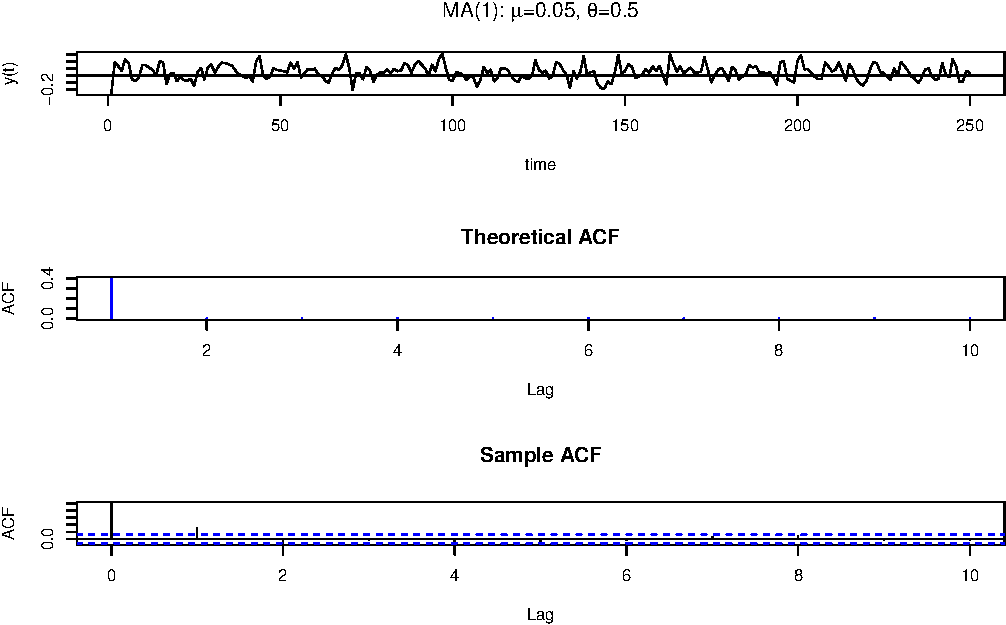
\includegraphics{homework_4_markdown_files/figure-latex/unnamed-chunk-2-1.pdf}
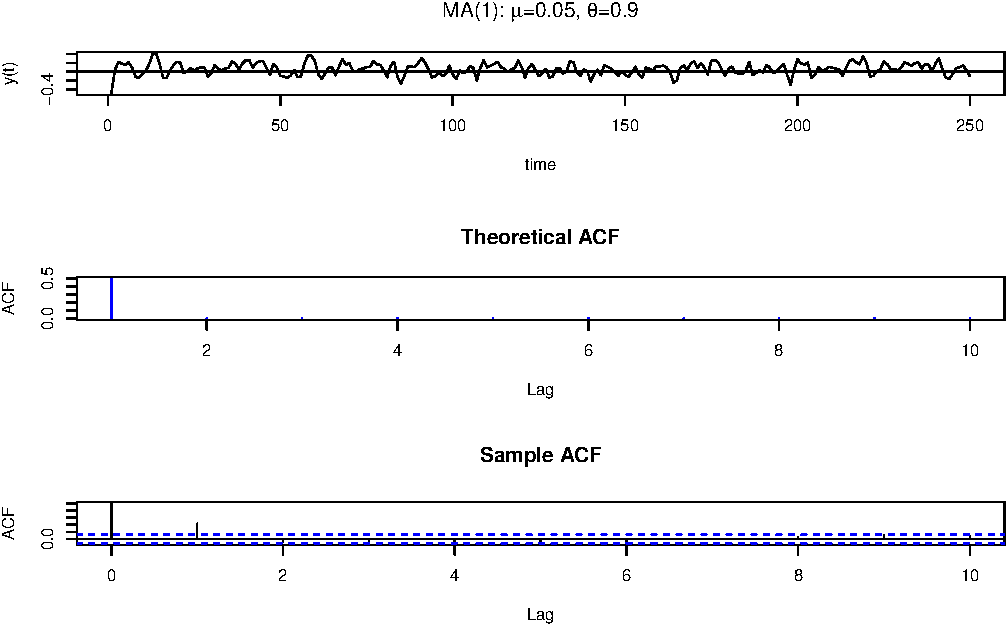
\includegraphics{homework_4_markdown_files/figure-latex/unnamed-chunk-2-2.pdf}
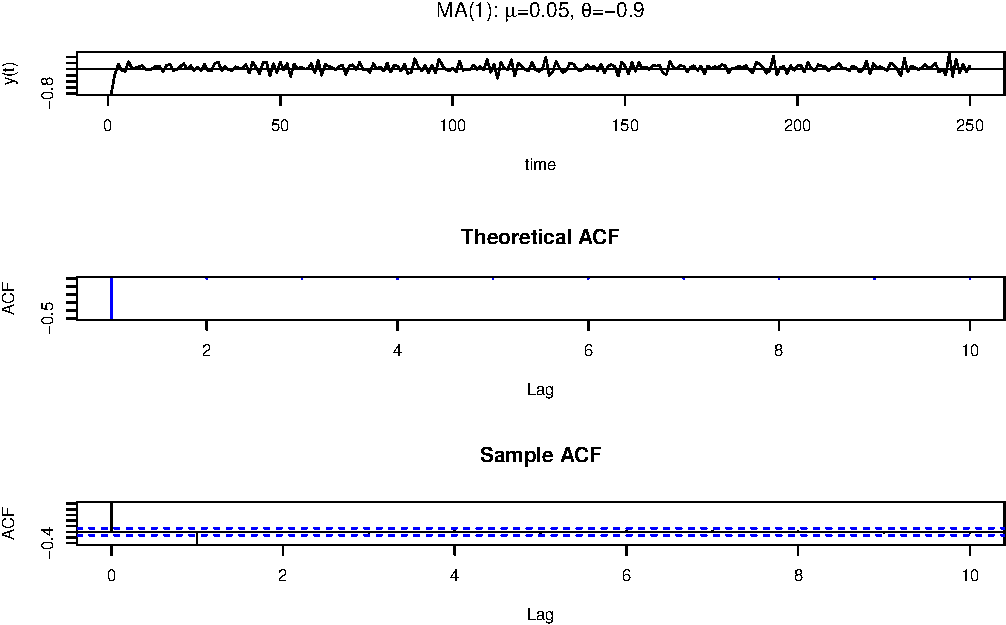
\includegraphics{homework_4_markdown_files/figure-latex/unnamed-chunk-2-3.pdf}

\paragraph{(b) Briefly comment on the behavior of the simulated data
series.}\label{b-briefly-comment-on-the-behavior-of-the-simulated-data-series.}

The MA(1) time series shows a spike of time dependence at one lag for
this simulation. The direction depends on the sign of \(\theta\) Note
that this spike is outside the confidence interval. Also, the higher
\(\theta\) can can result in a lower or higher than usual first point in
the series.

\subsubsection{1. Consider the AR(1)
model}\label{consider-the-ar1-model}

\paragraph{\texorpdfstring{(a) Using the R function arima.sim(),
simulate and plot 250 observations of the AR(1) with \(\phi\)=0,
\(\phi\)=0.5, \(\phi\)=0.9 and
\(\phi\)=0.99.}{(a) Using the R function arima.sim(), simulate and plot 250 observations of the AR(1) with \textbackslash{}phi=0, \textbackslash{}phi=0.5, \textbackslash{}phi=0.9 and \textbackslash{}phi=0.99.}}\label{a-using-the-r-function-arima.sim-simulate-and-plot-250-observations-of-the-ar1-with-phi0-phi0.5-phi0.9-and-phi0.99.}

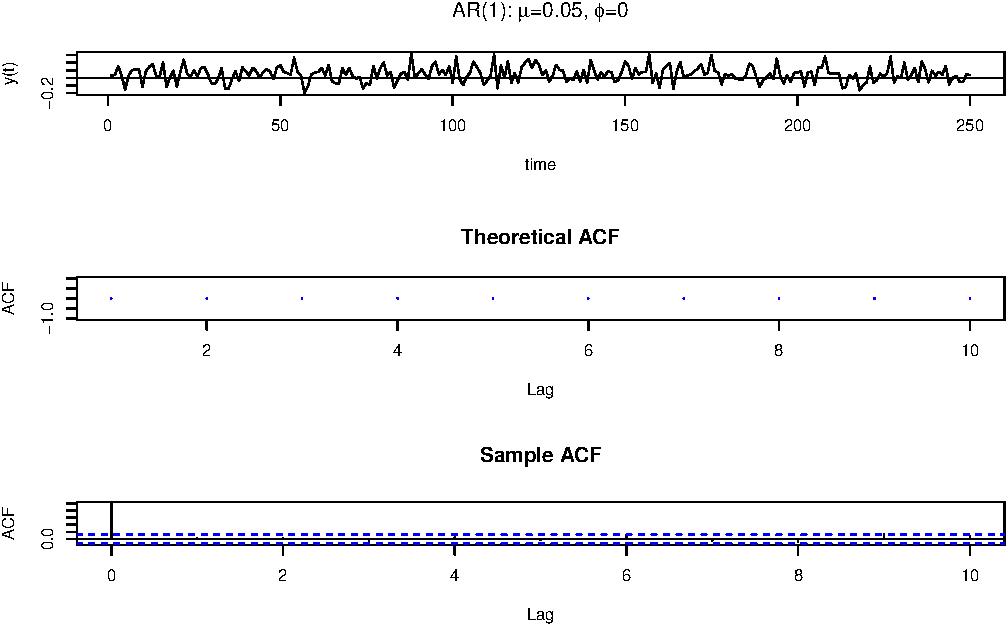
\includegraphics{homework_4_markdown_files/figure-latex/unnamed-chunk-3-1.pdf}
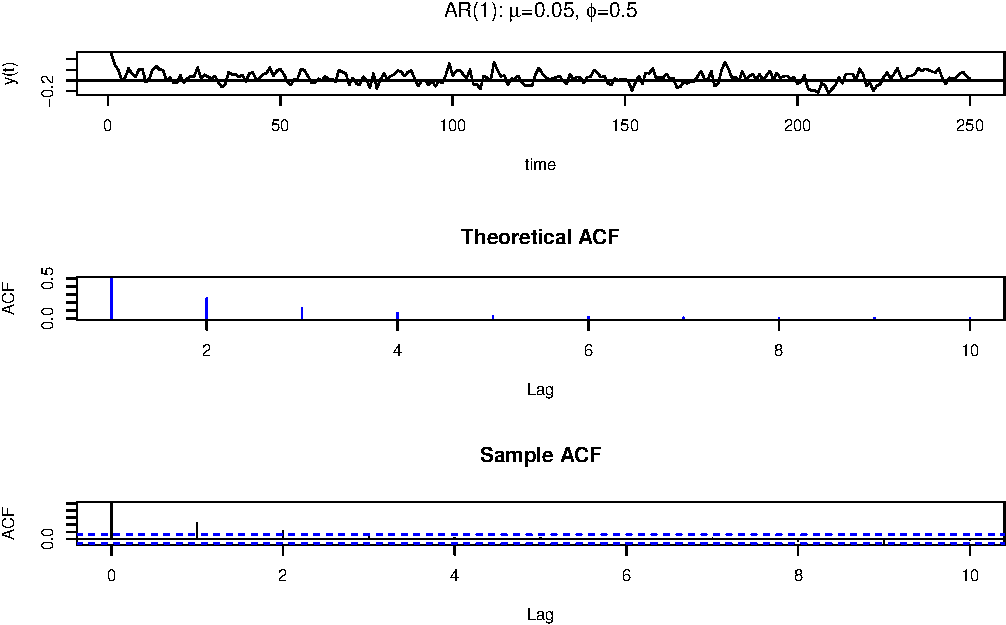
\includegraphics{homework_4_markdown_files/figure-latex/unnamed-chunk-3-2.pdf}
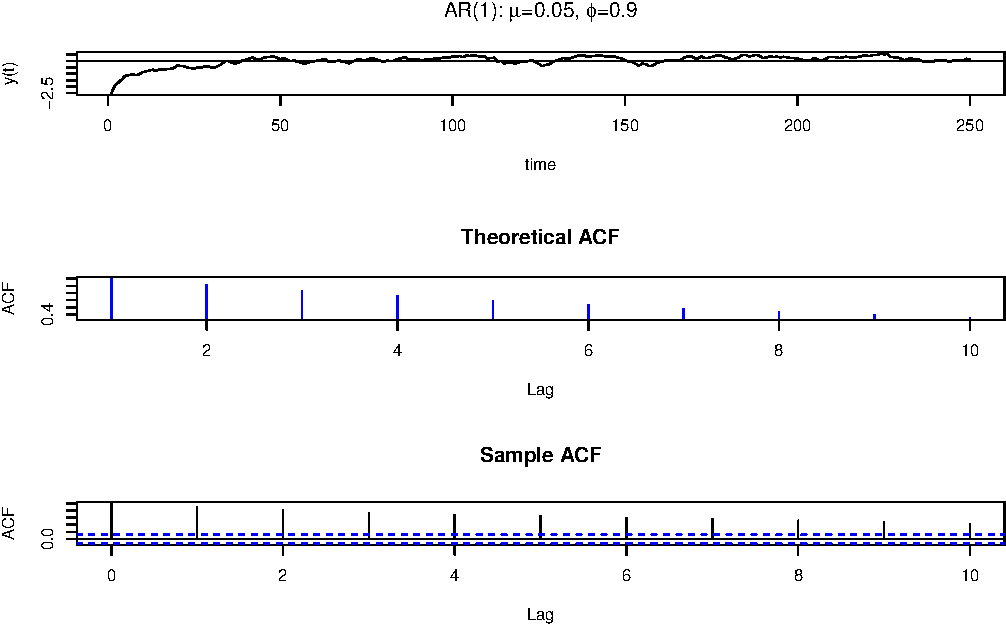
\includegraphics{homework_4_markdown_files/figure-latex/unnamed-chunk-3-3.pdf}
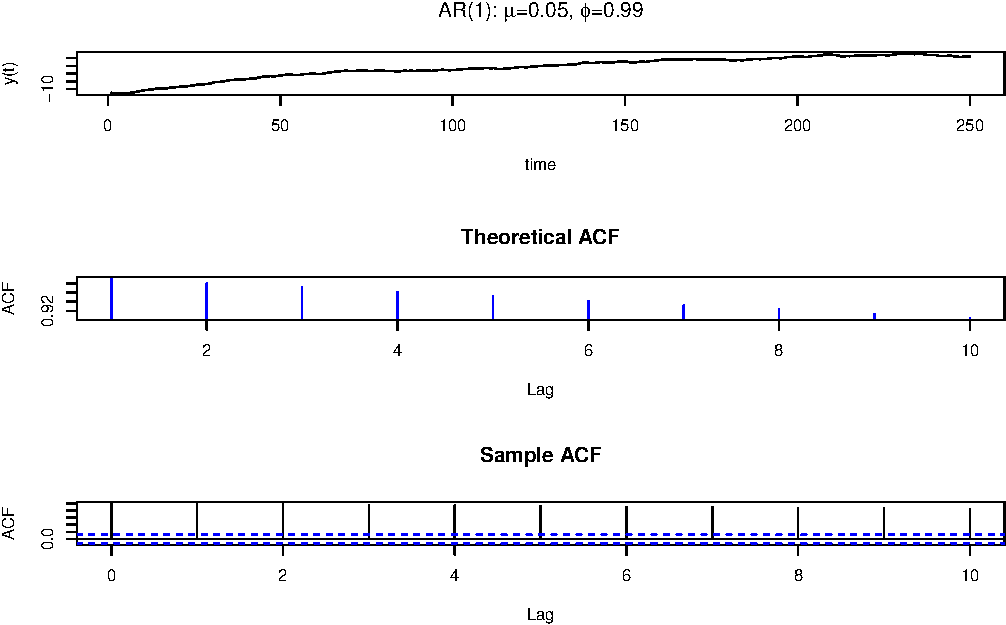
\includegraphics{homework_4_markdown_files/figure-latex/unnamed-chunk-3-4.pdf}

\paragraph{(b) Comment on the behavior of the simulated data series.
Which series is close to nonstationary (or persistent) time
series?}\label{b-comment-on-the-behavior-of-the-simulated-data-series.-which-series-is-close-to-nonstationary-or-persistent-time-series}

The AR(1) time series shows time dependence that decays slowly over
time. We can observe that the higher phi associates with stronger
persistence. However, when it gets too close to 1 it becomes like a
nonstationary process.

\subsection{R Exercises B}\label{r-exercises-b}

\subsubsection{0. Briefly discuss what these assets are (VBLTX, FMAGX
and
SBUX)}\label{briefly-discuss-what-these-assets-are-vbltx-fmagx-and-sbux}

VBLTX is the Vanguard Long-Term Bond Index mutual fund, FMAGX is the
Fidelity Magellan Fund, and SBUX is Starbucks stock.

\subsubsection{1. (Descriptive Statistics) Do the following replication
exercises.}\label{descriptive-statistics-do-the-following-replication-exercises.}

\paragraph{(a) Make time plots of the returns. Comment on any
relationships between the returns suggested by the plots. Pay particular
attention to the behavior of returns toward the end of 2008 at the
beginning of the financial
crisis.}\label{a-make-time-plots-of-the-returns.-comment-on-any-relationships-between-the-returns-suggested-by-the-plots.-pay-particular-attention-to-the-behavior-of-returns-toward-the-end-of-2008-at-the-beginning-of-the-financial-crisis.}

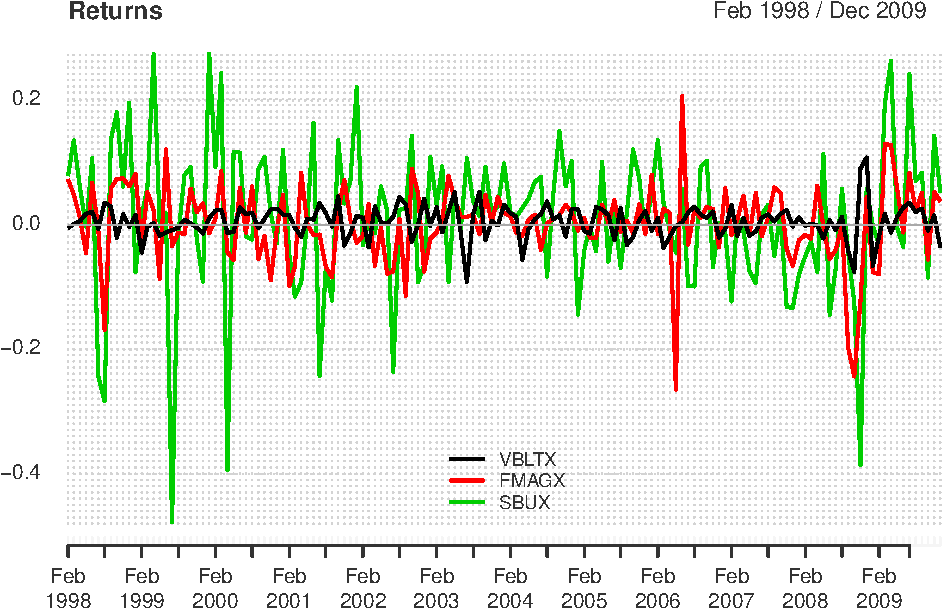
\includegraphics{homework_4_markdown_files/figure-latex/unnamed-chunk-5-1.pdf}

All time series appear to be stationary with varying levels of
volatility. There is more volatility towards the financial crisis,
especially in SBUX and FMAGX.

\paragraph{(b) Make a cumulative return plot (future of \$1 invested in
each asset) and comment. Which assets gave the best and worst future
values over the investment
horizon?}\label{b-make-a-cumulative-return-plot-future-of-1-invested-in-each-asset-and-comment.-which-assets-gave-the-best-and-worst-future-values-over-the-investment-horizon}

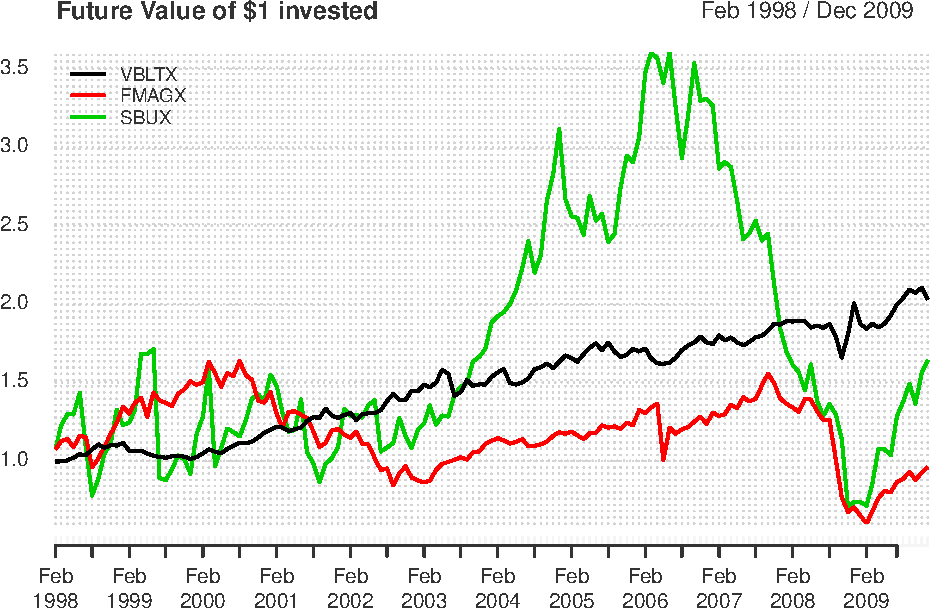
\includegraphics{homework_4_markdown_files/figure-latex/unnamed-chunk-6-1.pdf}

From this plot, the VBLTX gave the best future value of the investment
at present time. But we also note that Starbucks had the highest value
around 3.5, before it dropped significantly in 2007. The FMAGX
consistently had the worst future values.

\paragraph{(c) For each return series, make a four panel plot containing
a histogram, density plot, boxplot and normal QQ-plot. Do the return
series look normally distributed? Briefly compare the return
distributions.}\label{c-for-each-return-series-make-a-four-panel-plot-containing-a-histogram-density-plot-boxplot-and-normal-qq-plot.-do-the-return-series-look-normally-distributed-briefly-compare-the-return-distributions.}

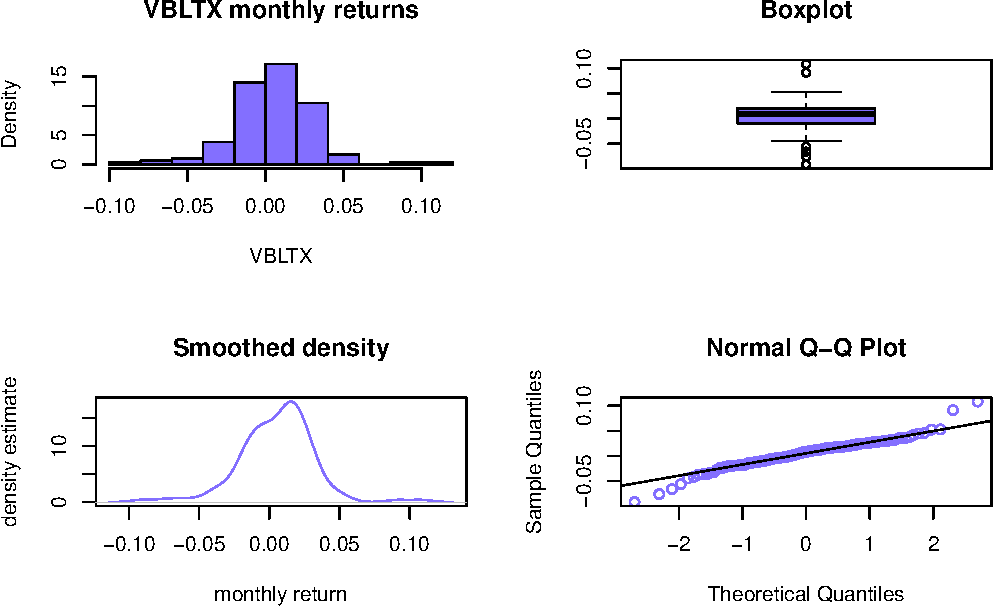
\includegraphics{homework_4_markdown_files/figure-latex/unnamed-chunk-7-1.pdf}
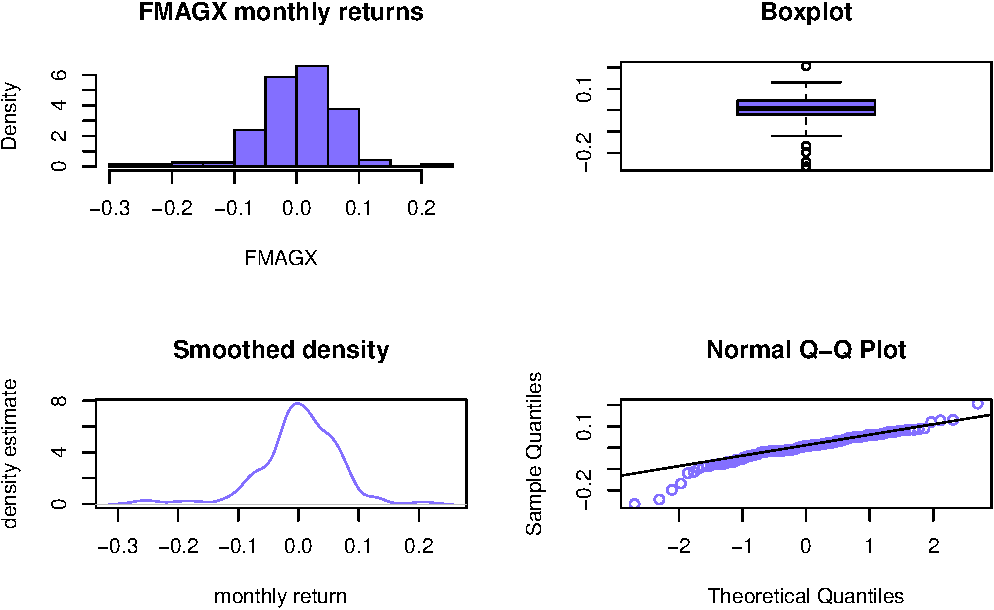
\includegraphics{homework_4_markdown_files/figure-latex/unnamed-chunk-7-2.pdf}
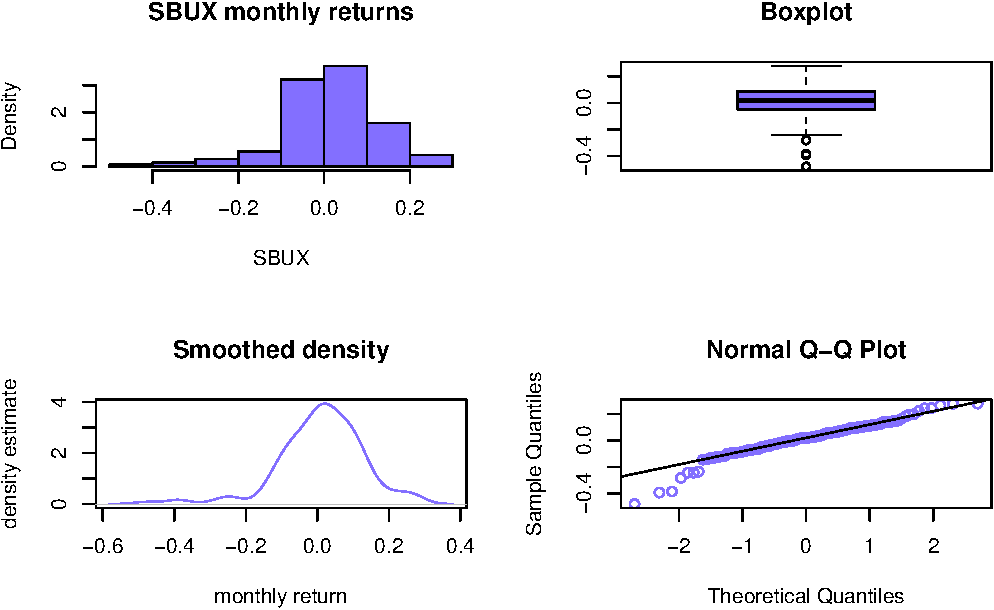
\includegraphics{homework_4_markdown_files/figure-latex/unnamed-chunk-7-3.pdf}
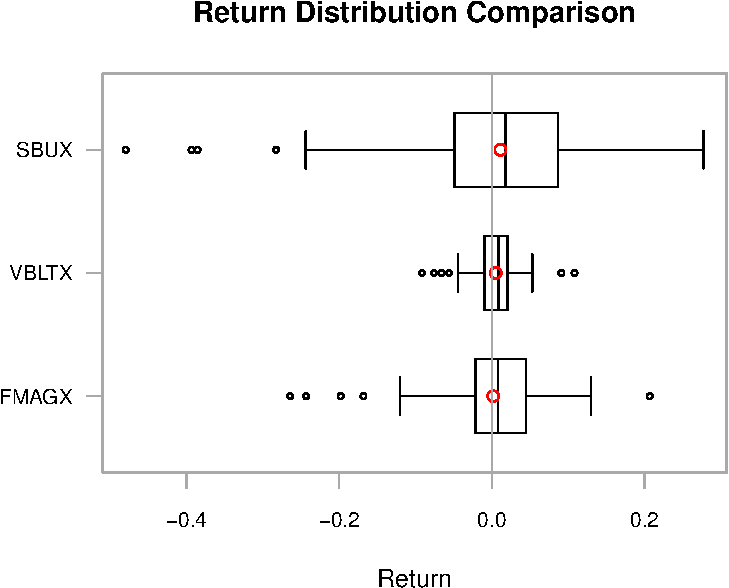
\includegraphics{homework_4_markdown_files/figure-latex/unnamed-chunk-7-4.pdf}

For the most part, the returns of these time series all look somewhat
normal. The QQ-Plots all show fatter tails than a normal distribution,
which is expected in financial return data. We can also see that
Starbucks has a slightly higher median value than zero.

\paragraph{(d) Compute numerical descriptive statistics for all assets
using the R functions summary(), mean(), var(), stdev(), skewness(), and
kurtosis() (in package PerformanceAnalytics). Compare and contrast the
descriptive statistics for the three assets. Which asset appears to be
the riskiest
asset?}\label{d-compute-numerical-descriptive-statistics-for-all-assets-using-the-r-functions-summary-mean-var-stdev-skewness-and-kurtosis-in-package-performanceanalytics.-compare-and-contrast-the-descriptive-statistics-for-the-three-assets.-which-asset-appears-to-be-the-riskiest-asset}

\begin{verbatim}
##                    VBLTX    FMAGX     SBUX
## Observations    143.0000 143.0000 143.0000
## NAs               0.0000   0.0000   0.0000
## Minimum          -0.0914  -0.2643  -0.4797
## Quartile 1       -0.0096  -0.0212  -0.0488
## Median            0.0086   0.0082   0.0182
## Arithmetic Mean   0.0053   0.0019   0.0113
## Geometric Mean    0.0050  -0.0003   0.0035
## Quartile 3        0.0204   0.0450   0.0868
## Maximum           0.1083   0.2069   0.2773
## SE Mean           0.0022   0.0054   0.0100
## LCL Mean (0.95)   0.0010  -0.0087  -0.0084
## UCL Mean (0.95)   0.0096   0.0125   0.0311
## Variance          0.0007   0.0041   0.0143
## Stdev             0.0263   0.0641   0.1194
## Skewness         -0.1470  -0.9284  -0.9061
## Kurtosis          2.8871   3.3977   2.6948
\end{verbatim}

Here we again see that SBUX has a median return of about 2\% while the
others are around 0.1\%. Starbucks also has the highest maximum value.
However, Starbuck's variance is at 0.01 while the other series are
0.0007 and 0.0041. All series have a slight negative skew, meaning
longer tails to the left than the right. Starbucks and VBLTX have lower
than normal Kurtosis and FMAGX has a higher kurtosis. From these results
we can see that Starbucks is the riskiest asset, but also has the chance
for highest return.

\paragraph{(e) Using the mean monthly return for each asset, compute an
estimate of the annual continuously compounded return (i.e., recall the
relationship between the expected monthly cc return and the expected
annual cc return). Convert this annual continuously compounded return
into a simple annual return. Are there any
surprises?}\label{e-using-the-mean-monthly-return-for-each-asset-compute-an-estimate-of-the-annual-continuously-compounded-return-i.e.-recall-the-relationship-between-the-expected-monthly-cc-return-and-the-expected-annual-cc-return.-convert-this-annual-continuously-compounded-return-into-a-simple-annual-return.-are-there-any-surprises}

\begin{verbatim}
##      VBLTX      FMAGX       SBUX 
## 0.06362524 0.02227371 0.13581968
\end{verbatim}

\begin{verbatim}
##      VBLTX      FMAGX       SBUX 
## 0.06569294 0.02252362 0.14547532
\end{verbatim}

Here we see Starbucks has the highest cc return at 0.14, with VBLTX in
second at 0.06 and FMAGX at 0.02. When we convert these to simple
returns all the values are slightly higher.

\paragraph{(f) Using the estimate of the monthly return standard
deviation for each asset, compute an estimate of the annual return
standard deviation. Briefly comment on the magnitude of the annual
standard
deviations.}\label{f-using-the-estimate-of-the-monthly-return-standard-deviation-for-each-asset-compute-an-estimate-of-the-annual-return-standard-deviation.-briefly-comment-on-the-magnitude-of-the-annual-standard-deviations.}

\begin{verbatim}
##      VBLTX      FMAGX       SBUX 
## 0.09101233 0.22201945 0.41358651
\end{verbatim}

Starbucks has the largest standard deviation. FMAGX and VBLTX have the
second and third largest standard deviations.

\paragraph{(g) Use the R pairs() function to create all pair-wise
scatterplots of returns. Comment on the direction and strength of the
linear relationships in these
plots.}\label{g-use-the-r-pairs-function-to-create-all-pair-wise-scatterplots-of-returns.-comment-on-the-direction-and-strength-of-the-linear-relationships-in-these-plots.}

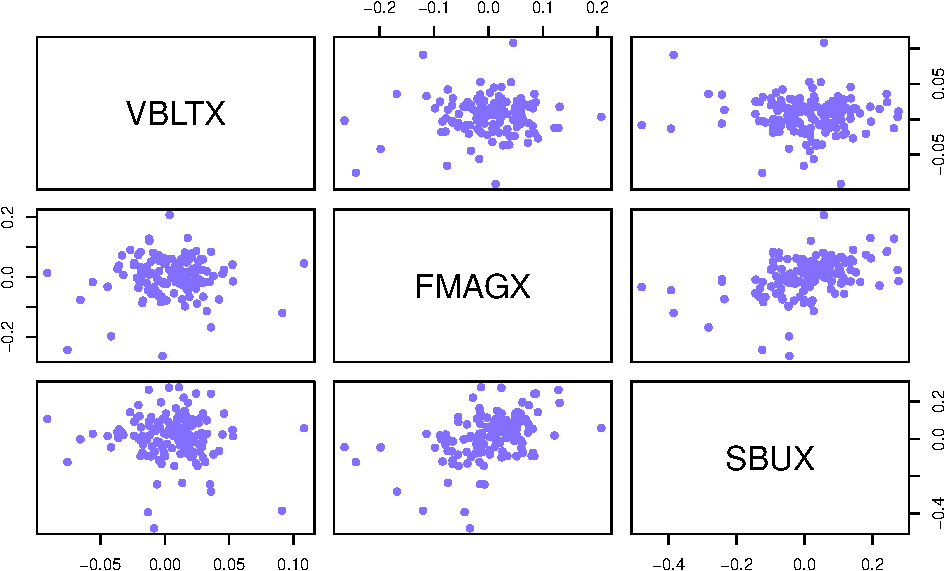
\includegraphics{homework_4_markdown_files/figure-latex/unnamed-chunk-11-1.pdf}

From our plot we can see that FMAGX and SBUX have a positive
association. FMAGX and VBLTX also appear to have weak positive
associations. VBLTX and SBUX seem to have a negative association. All of
these relationships look somewhat weak, with the exception of VBLTX and
SBUX.

\paragraph{(h) Use the R functions var() and cor() to compute the sample
covariance matrix and sample correlation matrix of the returns. Comment
on the direction and strength of the linear relationships suggested by
the values of the covariances and
correlations.}\label{h-use-the-r-functions-var-and-cor-to-compute-the-sample-covariance-matrix-and-sample-correlation-matrix-of-the-returns.-comment-on-the-direction-and-strength-of-the-linear-relationships-suggested-by-the-values-of-the-covariances-and-correlations.}

\begin{verbatim}
##               VBLTX        FMAGX          SBUX
## VBLTX  0.0006902704 0.0001073546 -0.0001761074
## FMAGX  0.0001073546 0.0041077197  0.0032432391
## SBUX  -0.0001761074 0.0032432391  0.0142544835
\end{verbatim}

\begin{verbatim}
##             VBLTX     FMAGX        SBUX
## VBLTX  1.00000000 0.0637545 -0.05614256
## FMAGX  0.06375450 1.0000000  0.42384085
## SBUX  -0.05614256 0.4238409  1.00000000
\end{verbatim}

The matrix tells us that FMAGX and VBLTX have a weak positive
correlation, VBLTX and SBUX have a weak negative correlation, and SBUX
and FMAGX have a moderate positive correlation.

\paragraph{(i) Use the R function acf() to compute and plot the sample
autocorrelation functions of each return. Do the returns appear to be
uncorrelated over
time?}\label{i-use-the-r-function-acf-to-compute-and-plot-the-sample-autocorrelation-functions-of-each-return.-do-the-returns-appear-to-be-uncorrelated-over-time}

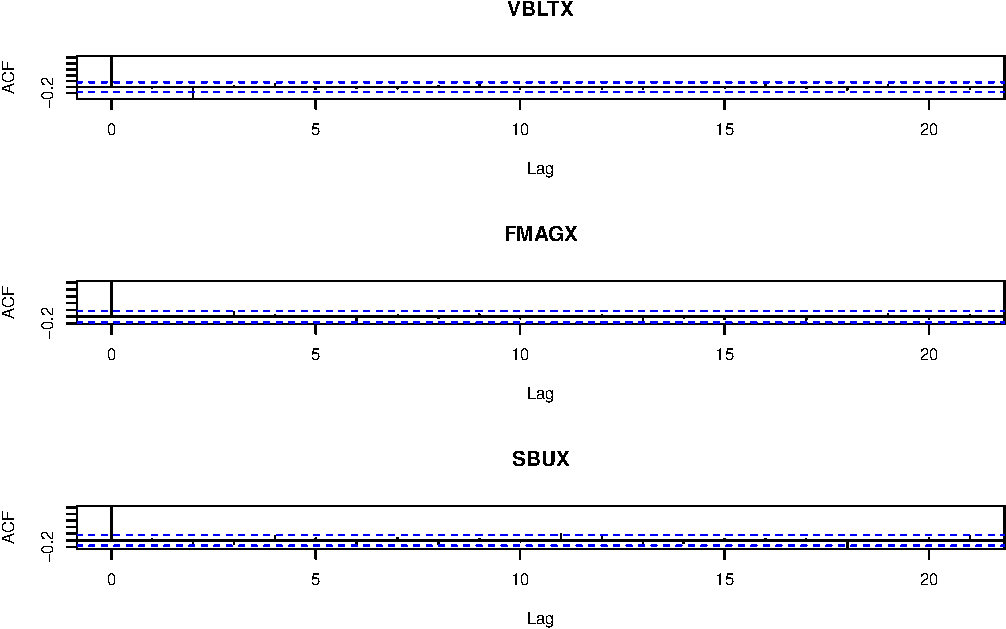
\includegraphics{homework_4_markdown_files/figure-latex/unnamed-chunk-13-1.pdf}

The ACF plots tell us that all the series are not time dependent. VBLTX
has one significat spike at lag 2 but this probably does not carry any
economic meaning and is due to chance.

\subsubsection{2. (IID Normal Model) Consider the IID normal
model}\label{iid-normal-model-consider-the-iid-normal-model}

\paragraph{(a) Using sample descriptive statistics, give estimates for
the model parameters. Arrange these estimates nicely in a table. Briefly
comment.}\label{a-using-sample-descriptive-statistics-give-estimates-for-the-model-parameters.-arrange-these-estimates-nicely-in-a-table.-briefly-comment.}

\begin{verbatim}
##        muhat.vals sigma2hat.vals sigmahat.vals
## VBLTX 0.005302103   0.0006902704    0.02627300
## FMAGX 0.001856142   0.0041077197    0.06409149
## SBUX  0.011318306   0.0142544835    0.11939214
\end{verbatim}

\begin{verbatim}
##               covhat.vals rhohat.vals
## VBLTX,FMAGX  0.0001073546  0.06375450
## VBLTX,SBUX  -0.0001761074 -0.05614256
## FMAGX,SBUX   0.0032432391  0.42384085
\end{verbatim}

Our estimates of these parameters all coincide with what we observed
earlier. SBUX has the highest mean value but also the largest
variance(risk). The covariane and correlation coefficients also indicate
the same relationships as noted earlier.

\paragraph{(b) For each estimate of the above parameters. Briefly
comment on the precision of the
estimates.}\label{b-for-each-estimate-of-the-above-parameters.-briefly-comment-on-the-precision-of-the-estimates.}

\begin{verbatim}
##        muhat.vals    se.muhat
## VBLTX 0.005302103 0.002197058
## FMAGX 0.001856142 0.005359600
## SBUX  0.011318306 0.009984072
\end{verbatim}

SBUX has the largest standard error at 0.009, FMAGX has the second
largest at 0.005, and VBLTX the lowest at 0.002.

\paragraph{(c) For each parameter compute 95\% and 99\% confidence
intervals. Briefly comment on the width of these
intervals.}\label{c-for-each-parameter-compute-95-and-99-confidence-intervals.-briefly-comment-on-the-width-of-these-intervals.}

\begin{verbatim}
##            mu.lower   mu.upper
## VBLTX  0.0009079864 0.00969622
## FMAGX -0.0088630580 0.01257534
## SBUX  -0.0086498385 0.03128645
\end{verbatim}

There are negative and positive values for the returns, which might
indicate bad estimation.

\begin{verbatim}
##       sigma2.lower sigma2.upper
## VBLTX 0.0005270042 0.0008535365
## FMAGX 0.0031361415 0.0050792980
## SBUX  0.0108829424 0.0176260246
\end{verbatim}

\begin{verbatim}
##       sigma.lower sigma.upper
## VBLTX  0.02316589  0.02938011
## FMAGX  0.05651188  0.07167111
## SBUX   0.10527253  0.13351175
\end{verbatim}

The SE for variance and SE are very narrow, which means good precision.

\begin{verbatim}
##             rhohat.vals  se.rhohat
## VBLTX,FMAGX  0.06375450 0.08328430
## VBLTX,SBUX  -0.05614256 0.08336062
## FMAGX,SBUX   0.42384085 0.06860186
\end{verbatim}

\begin{verbatim}
##              rho.lower rho.upper
## VBLTX,FMAGX -0.1028141 0.2303231
## VBLTX,SBUX  -0.2228638 0.1105787
## FMAGX,SBUX   0.2866371 0.5610446
\end{verbatim}

These intervals for the top 2 are somewhat wide and between negative and
positive numbers. The bottom row looks narrower and on the same side of
zero.

\paragraph{(d) Compute the 1\% and 5\% monthly value-at-Risk (VaR) based
on an initial \$100,000 investment. Which fund has the lowest
VaR?}\label{d-compute-the-1-and-5-monthly-value-at-risk-var-based-on-an-initial-100000-investment.-which-fund-has-the-lowest-var}

\begin{verbatim}
##      VBLTX      FMAGX       SBUX 
##  -3720.343  -9838.257 -16894.915
\end{verbatim}

\begin{verbatim}
##      VBLTX      FMAGX       SBUX 
##  -5428.879 -13691.575 -23388.987
\end{verbatim}

The VBLTX fund has the lowest VaR, and SBUX has the highest VaR.


\end{document}
